\section{2-D plots}

{\setbeamercolor{background canvas}{bg=LemonChiffon}
\begin{frame}
\frametitle{}
{\fontsize{40}{50}\selectfont Programming in Python \#2} 

{\huge 2D plots and plots on map} 

\end{frame}
}

%--------------------------------------------------------------------------------------------------------------
\begin{frame}
\frametitle{Useful packages}

\begin{description}
\item<1->[NumPy:] package for scientific computing \url{http://www.numpy.org/}
\item<1->[SciPy:] open-source software for mathematics, science, and engineering \url{http://www.scipy.org/}
\item<2->[matplotlib:] 2D plotting library which produces publication quality figures \url{http://matplotlib.org/}
\item<3->[Basemap toolkit]: library for plotting 2D data on maps in Python \url{http://matplotlib.org/basemap/}
\item[]
\item<4->[Bokeh:] interactive visualization library (\url{http://bokeh.pydata.org/en/latest/}) 
\end{description}
\end{frame}

%--------------------------------------------------------------------------------------------------------------

\begin{frame}[c, fragile]
\frametitle{List of notebooks}

Located in \verb|Plotting|

{
\scriptsize
\begin{description}
\item[plot2D\_contours\_pcolor.ipynb:] plot 2D fields with contour or pseudo-color techniques       
\item[]
\item[plot2D\_map\_field.ipynb:] plot 2D field on a map              
\item[plot2D\_map\_vector.ipynb:] plot vector field on a map
\item[plot2D\_map\_scatter.ipynb:] scatter plot on a map
\end{description}
}

\begin{figure}
\includegraphics[height=2.5cm]{temperature_model}~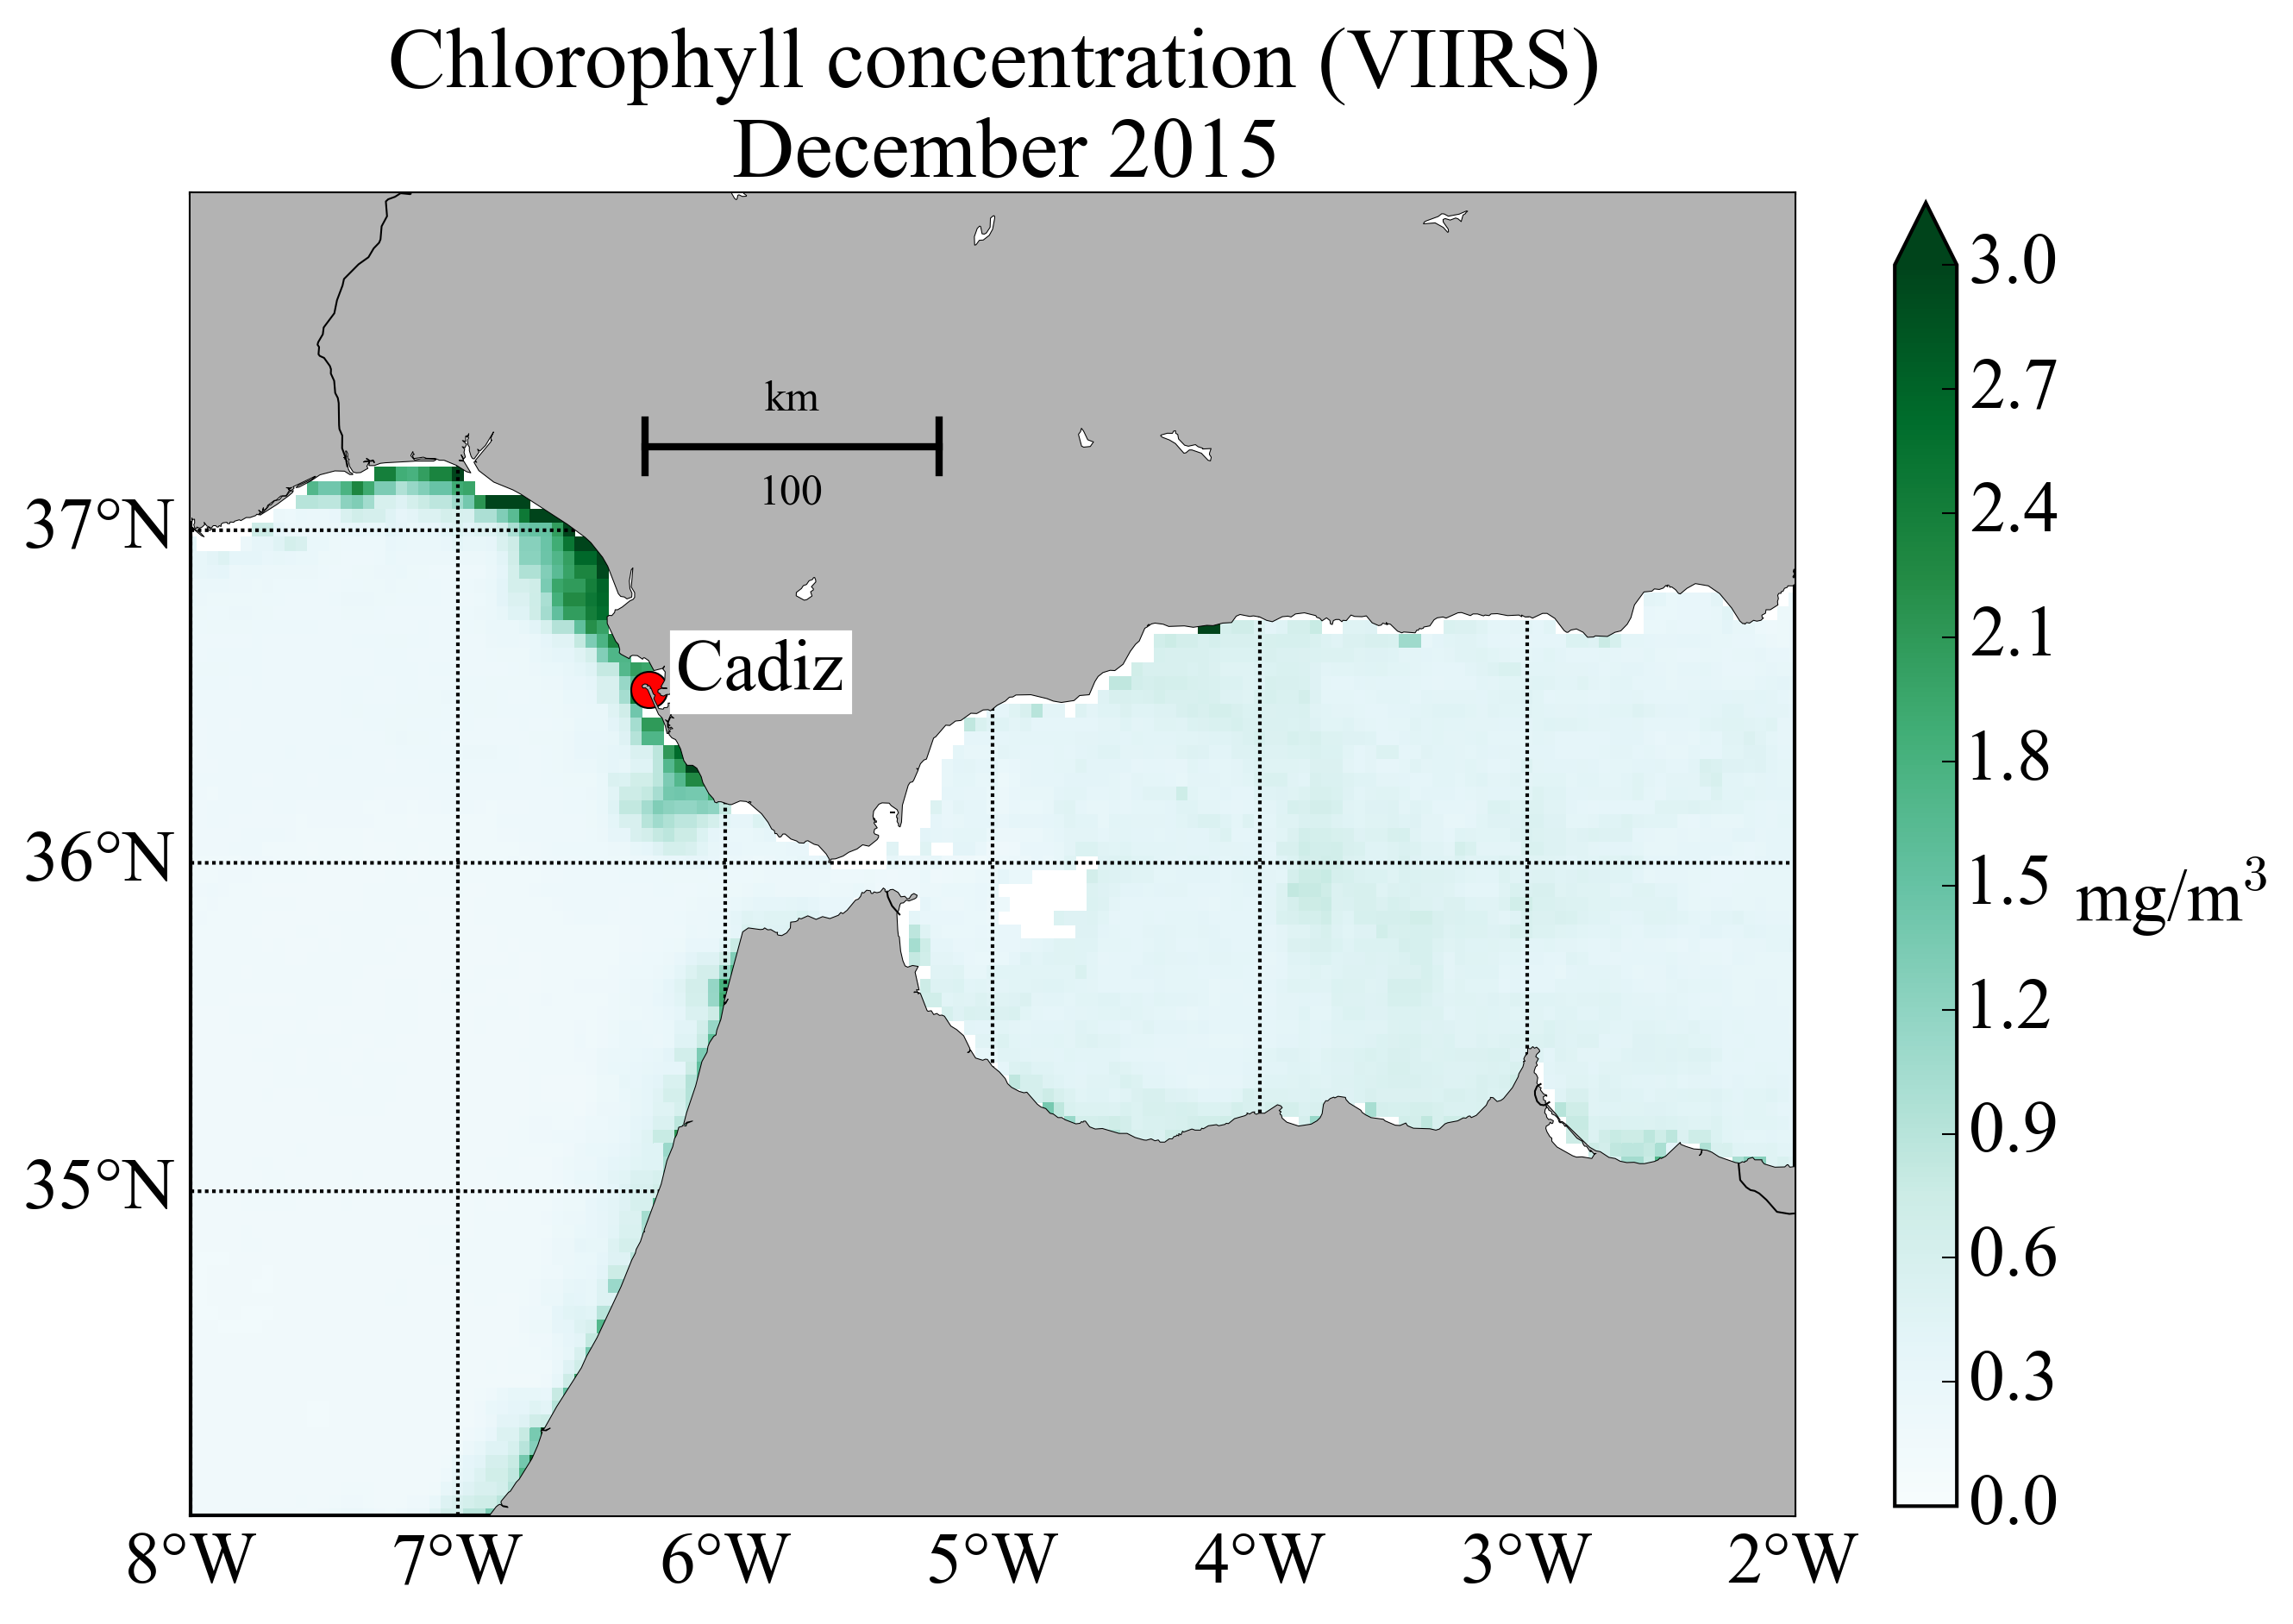
\includegraphics[height=2.5cm]{chloro201512_map}~\includegraphics[height=2.5cm]{radar_pde}
\end{figure}
\end{frame}

%--------------------------------------------------------------------------------------------------------------
\begin{frame}[c, fragile]
\frametitle{Exercise 3: 2D plot}

\textbf{Objective:} create a plot with the salinity from a numerical model and the velocities taken from a HF radar system.

\vspace{1cm}

\exercise \verb|3-plot_radar_salinity.ipynb|

\end{frame}